\section{Построение кривой Безье}

На рис.~\ref{picture-bezier-plane} изображена кривая Безье на плоскости, построенная по набору точек. Можно видеть
отрезки, последовательно соединяющие точки $p_i$, и точки $q_i$, являющиеся серединами этих отрезков. Также здесь
наглядно показан результат сглаживания последовательных пар отрезков.

\begin{figure}[h!]
\center{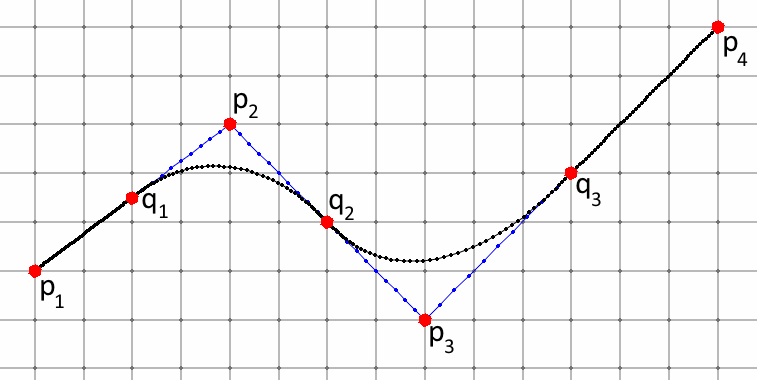
\includegraphics[scale=0.85]{bezier-plane}}
\caption{Построение кривой Безье на плоскости}
\label{picture-bezier-plane}
\end{figure}

На рис.~\ref{picture-bezier-two-dimension} изображена кривая Безье на поверхности двумерной сферы, построенная
по набору точек. Здесь, по аналогии с предыдущим изображением, можно видеть, что каждые две последовательные точки
на поверхности сферы соединены большими дугами. Дуги поделены пополам, и две точки, являющиеся их серединами,
соединены кривой, построенной как результат сглаживания двух участков больших дуг.

\begin{figure}[h!]
\center{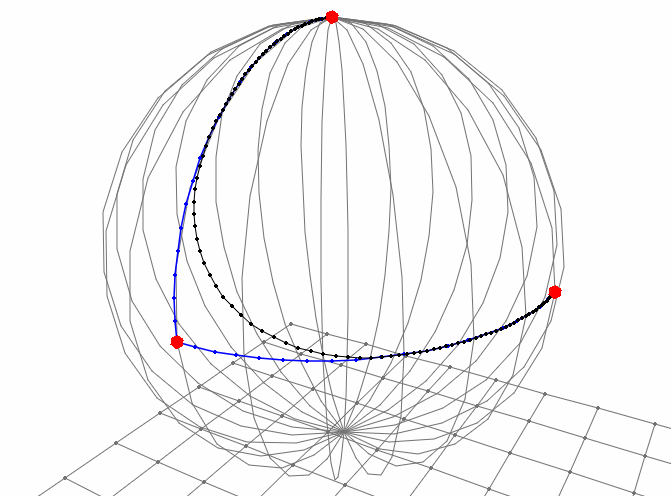
\includegraphics[scale=0.95]{bezier-two-dimension}}
\caption{Построение кривой Безье на двумерной сфере}
\label{picture-bezier-two-dimension}
\end{figure}

На рис.~\ref{picture-bezier-orientation} можно видеть набор ориентаций 3D-объекта. Чёрным выделен объект
в изначальном положении. Чёрная кривая "--- это тот путь, который пройдёт самая верхняя точка объекта при
воспроизведении построенной анимации. Каждые две последовательные ориентации соединены большими дугами, лежащими
на ориентационной сфере и поделенными пополам. Середины этих дуг соединены результатом сглаживания участков дуг.
Этот участок можно увидеть на рисунке у средней ориентации. Там анимация построена так, что через эту ориентацию объект
не проходит.

\begin{figure}[t!]
\center{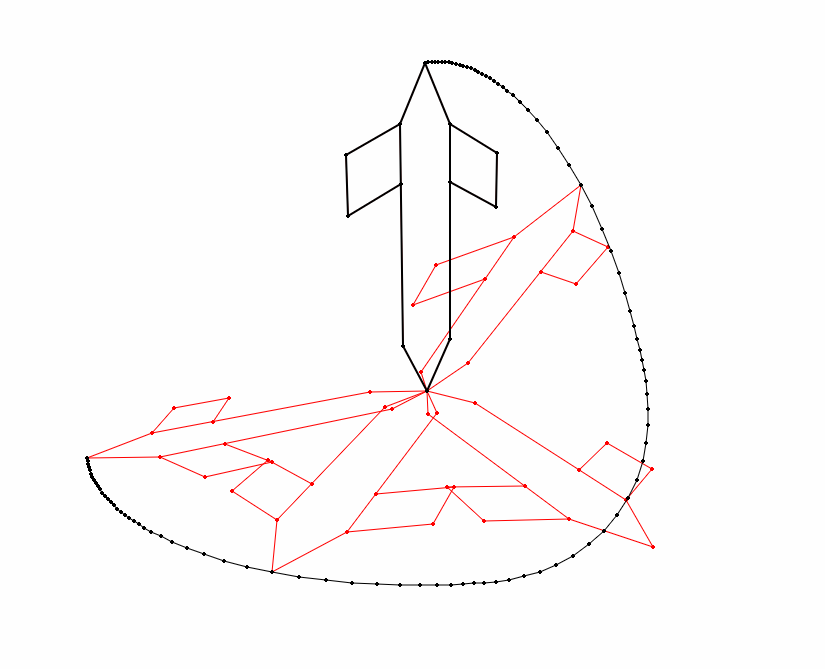
\includegraphics[scale=0.7]{bezier-orientation}}
\caption{Построение кривой Безье на ориентационной сфере}
\label{picture-bezier-orientation}
\end{figure}
